\subsubsection{Evaluation verfügbarer Produkte}
\label{sec:produkt-eval}
\paragraph{Auswahl der \ac{waf}-Anwendung}

\paragraph{Verwundbare Anwendungen}

\subsubsection{Labor-Umgebung}

% 1. Anforderungen an die Lernumgebung
% 2. Überlegungen zur gestaltung einheiltichen Deployments
% 2.1. Docker
%       - einheitlich
%       - Netzwerke
%       - Probleme mit croscompatibility (Windows)
% 2.2. VM (vortiele und Probleme)
% 3. beschreibung der Container
% 3.1. Juicesop
% 3.2. WAF
% 3.3. Python contaienr mit test script

Die in Kapitel \ref{sec:inhalte} beschriebenen Inhalte sollen in einem Praxisnahen Umfeld vermittelt werden.
Dazu kommt nach den Abwägungen aus Kapitel \ref{sec:produkt-eval}, die Waf-Applikation ModSecurity zum Einsatz.
Die zu diesem Zweck vorgesehene Laborumgebung muss einige Kriterien erfüllen:
\begin{description}
    \item[Einheitliches Deployment:] Der Ausgangspunkt der Lerneinheiten muss reproduzierbar und wiederholbar sein. 
    Bei wiederholten Durchführungen der Übungen soll es einfach sein den Lernenden ohne zusätzlichem manuellen Konfigurationsaufwand eine Laborumgebung zu übergeben. 
    Diese Laborumgebung muss Platform-unabhängig aufgebaut sein und auf Windows, MacOS unf Linux genutzt werden können.
    \item[Modifizierbarketit der Anwendungen:] Um in den Lerneinheiten grundlegende Techniken zu übermitteln, ist es notwendig Basis-Funktion der ModSecurity \ac{waf} entfernen zu können. 
    Dies muss automatisierten und einheitlichen Weg erfolgen können.
    \item[Bekannte Basis-Technologien:] Der Fokus der Lerneinheiten liegt auf dem Erlernen der Technik und Funktion einer \ac{waf}. 
    Um einen Einstieg möglichst direkt zu gestalten sollen hierfür Technologien zuj Einsatz kommen, die den Lernenden schon bekannt sind und keinen zusätzlichen Lernaufwand erzeugen.
    \item[Komplexe Netzwerkumgebungen:] Da die verschiedenen Anwendungen in der Laborumgebung über Netzwerkkommunikation miteinander kommunizieren, muss es möglich sein automatisiert virtuelle Netzwerke zu erzeugen.
\end{description}

Um den oben genannten Anforderungen möglichst genau zu entsprechen, wurde die in Abbildung \ref{fig:lab} schematisch dargestellte Umgebung erstellt.

\begin{figure}[!hbt]
    \centering
    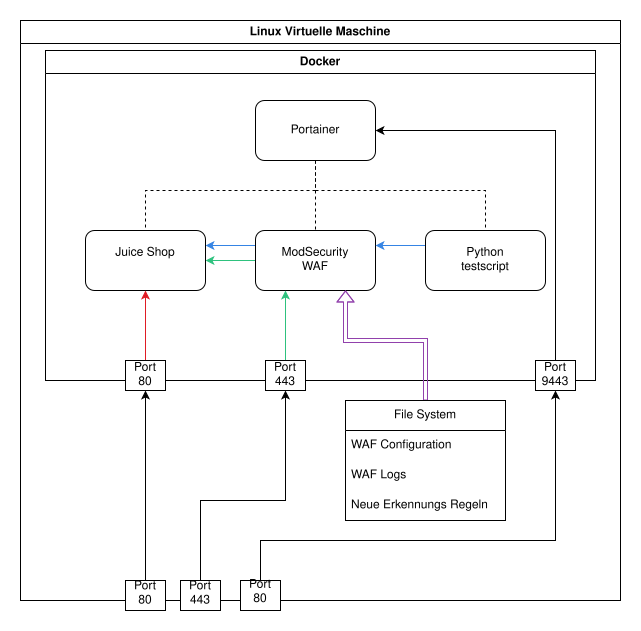
\includegraphics[width=0.9\textwidth]{./images/lab-setup.png}
    \caption{Aufbau der Laborumgebung}
    \label{fig:lab}
\end{figure}

Als Basis wird die Containervirtualisierungsumgebung Docker verwendet.
Diese ermöglicht es isolierte Ausführungsumgebungen für die Anwendungen zu erzeugen.
Der Aufbau dieser Umgebungen lässt sich mittels einer Konfigurationsdatei genau beschreiben und wiederholbar ausrollen.
Innerhalb der Umgebungen lässt sich festlegen wie die einzelnen Anwendungen (Container) untereinander kommunizieren und virtuelle Netzwerke anlegen um die Kommunikation zu isolieren.
Außerdem können Dateien oder Ordner aus dem Host-Dateisystem in den Container übergeben werden.
Dies ermöglicht es Konfigurationsdateien zu Verfügung zu stellen und somit, die sonst Status-losen Container, anzupassen.
Im Gegensatz zu virtuellen Maschinen greift die Containervirtualisierungsumgebung direkt auf die Mittel des Host-Betriebssystem zu und benötigt dadurch deutlich weniger Rechenaufwand.\\
\ \\
Wie in Abbildung \ref{fig:lab} dargestellt werden in der Laborumgebung vier Container betrieben:
\begin{description}
    \item[ModSecurity \ac{waf}:] Der Hersteller der in der Laborumgebung verwendeten \ac{waf} - ModSecurity - stellt sein Produkt auch in Form eines Docker-Containers zur Verfügung. 
    Diese wird jedoch in modifizierter Form genutzt.
    Da die \ac{waf} mit einer großen Anzahl vorkonfigurierten Regeln ausgeliefert wird, die für die meisten Aufgaben schon eine Lösung enthalten würden, müssen diese entfernt werden.
    An dessen Stelle wird ein Verzeichnis aus dem Host-Dateisystem durchgereicht in dem die Lernenden eigene Konfigurationen Platzieren können.
    Daneben werden, um das Debugging zu ermöglichen, die Log-Dateien aus der \ac{waf} im Host betriebssystem zur Verfügung gestellt.ds
    
    \item[Juice Shop:] Dieser wird in Version 16.0.0 verwendet, da der Hersteller (OWASP) die Anwendung regelmäßig verändert.
    Durch die Verwendung der neuesten Version könnten Challenges verloren gehen, die für die Durchführung der Aufgaben notwendig wäre.
    Auch diese Anwendung wird in modifizierter Form Ausgeliefert.
    Es werden Daten hinterlegt und Nutzeracounts angelegt.
    Diese ermöglichen es Mittels eines automatischen Kontroll-Scriptes die Konfiguration der \ac{waf} zu überprüfen.
    Die genauen Änderungen werden in den Sub-Kapiteln von Kapitel \ref{sec:learnings} im Detail beschrieben.

    \item[Python Test-Script:] Dieser Container enthält ein Python Skript, das es den Lernenden mittels des Unittest-Frameworks \textit{Pytest} ermöglicht, die erarbeiteten Lösungen zu überprüfen.
    Das Skript schickt HTTP-Requests durch die \ac{waf} und evaluiert die Antworten um den Lernenden Rückmeldung über den Erfolg ihrer Kofiguyration zu geben.
    Die jeweilige Funktion wird in den Sub-Kapiteln von Kapitel \ref{sec:learnings} im Detail beschrieben.

    \item[Portainer:] Die Anwendung \textit{Portainer} ermöglicht es eine Docker Umgebung mittels einer Grafischen Oberfläche zu verwalten.
    In der Laborumgebung kann sie genutzt werden um die Laborumgebung zu bedienen ohne sich tiefer mit der Funtion von Docker auseinander setzen zu müssen.
    Zwar können die Lernenden dies auch über das Docker Komandozeilen-Interface tun, jedoch beurteile ich dies als eine vermeidbare Hürde, die den Einstieg erschweren könnte.
    Die grafische Oberfläche soll unter anderem genutzt werden um des \ac{waf} kontainer nach einer Konfigurationsänderung neu zu starten und mit dem Test Skript zu interagieren. 
\end{description}
\ \\
Aus den oben genannten Containern ergeben sich einige Netz die im Hintergrund existieren müssen.
So ist es notwendig das von dem Python Test-Container zur \ac{waf} und von dieser eine Verbindung zum Jucice Shop aufgebaut werden muss.
Hierfür werden separate Docker-Netzwerke erstellt die an den Containern angeschlossen sind.
Um den Nutzern eine Interaktion mit den Containern zu ermöglichen werden einige Ports aus der Docker-Umgebung freigegeben:

\begin{itemize}
    \item Die Weboberfläche des Juice Shops (Port 80 [HTTP])
    \item Die, durch die \ac{waf} gesicherte, Weboberfläche des Juice Shops (Port 443 [HTTPS])
    \item Das Management Interface der Portainer-Anwendung (Port 8443 ][HTTPS])
\end{itemize}

Durch die oben beschriebene Docker Umgebung sind Anforderungen an die Laborumgebung wie dem \textit{einheitlichen Deployment} und der \textit{Modifizierbarketit der Anwendungen} bereits erfüllt.
Es ergeben sich jedoch auch einige Herausforderungen:
Docker ist zwar als Cross-Platform Anwendung konzipiert.
Es stehen Versionen für die drei Gängigen Betriebssysteme Windows, MacOS und Linux zur Verfügung.
Jedoch bauen die verwendeten Container Hauptsächlich auf Linux auf.
In der Theorie sollte dies zu keinen Problemen führen, da Docker in der Lage ist nicht Platform-Native Container auf sich unterscheidenden Betriebssystemen auszufühen, jedoch kann ein solcher Aufbau durchaus zu unvorhergesehenen Problemen führen.
Ein weiteres Problem ist, dass durch das Durchreichten von Dateien zwischen Container und dem Host-Dateisystem zusätzlicher Konfigurationsaufwand für die Nutzer entsehen könnte.

Um diesen Problemen Vorzubeugen wird die Laborumgebung als Linux Virtuelle Maschine ausgeliefert.
In dieser ist eine Docker Umgebung vorinstalliert und die Containerumgebung bereits präsent und wird automatisch gestartet.
Dies ermöglicht die Auslieferung mittels einer VM-Datei, in der die Konfigurationen schon an einer einheitlichen Stelle enthalten sind.
Lernende müssen zur Nutzung also nur eine Virtuelle Maschinen auf ihren Rechnern importieren und mittels eines Virtuellen Netzwerk Interface auf die Weboberflächen zugreifen.
Die Konfiguration der \ac{waf} findet in Textdateien statt, die sich in der Virtuellen Maschine befinden.
Der Zugriff auf diese ist mit dem Text-Editor Visual Studio Code der Firma Microsoft vorgesehen, da dieser eine SSH Erweiterung hat die es mit geringen Konfigurationsaufwand ermöglicht Dateien auf entfernten Servern oder in Virtuellen Maschinen zu bearbeiten.

Die Nutzung der Laborumgebung halte ich durch diese Maßnahmen für einfach genug um einen schnellen einstieg zu Ermöglichen.
Die Konfigurationen, die vorgenommen werden müssen, werden in der Ersten Lerneinhiet (Kapitel \ref{sec:lerneinheit1}) Beschrieben.
Es steht den Lernenden frei weitere oder andere als die beschriebenen Technologien zu verweden um mit der Laborumgebung zu interagieren.
Diese können im Rahmen dieser Thesis und den Aufgabenstellungen jehdoch nicht berücksichtigt werden.

\pagebreak